% vi:ft=tex
\documentclass{standalone}

\usepackage{tikz}
\usepackage{verbatim}

\usetikzlibrary{arrows}
\usetikzlibrary{calc}

\begin{document}

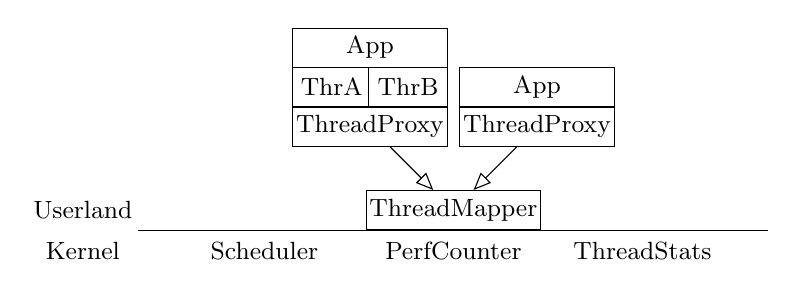
\begin{tikzpicture}[node distance=1.5cm]

  % Colors
  % Styles
  \tikzstyle{defaultRec} = [font=\small, text centered, inner sep = 1pt,
    draw=none, shape=rectangle, fill=white, minimum height = .5cm, minimum
  width = 1.4cm, text=black];
  \tikzstyle{tpRec} = [defaultRec, draw=black,text width=1.9cm];
  \tikzstyle{threadRec} = [defaultRec, draw=black, node distance=0mm,
  minimum width=1cm]
  \tikzstyle{arrow} = [-open triangle 45, black];

  % Variables

  % Drawing

  \draw[black, thin] (0,0) -- (8,0)
      node[defaultRec, above,pos=0,anchor=south east] {Userland}
      node(tm) [defaultRec, draw, above, pos=.5] {ThreadMapper}
      node[defaultRec,below,pos=0,anchor=north east] {Kernel}
      node[defaultRec, below, pos=.2] {Scheduler}
      node[defaultRec, below, pos=.5] {PerfCounter}
      node[defaultRec, below, pos=.8] {ThreadStats};

      \node(tp1) [tpRec, above left of=tm] {ThreadProxy};
      \draw[transparent] (tp1.west) -- +(0,5mm) coordinate(helpWest);
      \node(t1.1) [threadRec, right of=helpWest,anchor=west,] {ThrA};

      \draw[transparent] (tp1.east) -- +(0,5mm) coordinate(helpEast);
      \node(t1.2) [threadRec, right of=helpEast,anchor=east,] {ThrB};

      \node(a1)	[tpRec, above of=tp1, node distance=1cm] {App};

      \node(tp2) [tpRec, above right of=tm] {ThreadProxy};
      \node(a2)	[tpRec, above of=tp2, node distance=5mm] {App};

      \draw [arrow] (tp1) to (tm);
      \draw [arrow] (tp2) to (tm);

\end{tikzpicture}

\end{document}
